\documentclass{article} % For LaTeX2e
\usepackage[legalpaper, margin=0.5in]{geometry}
\usepackage{amsmath}
\usepackage{amsfonts,dsfont}
\usepackage{amssymb}
\usepackage[ruled,vlined]{algorithm2e}

\usepackage{graphicx}
\usepackage{caption}
\usepackage{subcaption}
\usepackage{xcolor}

\begin{document}

\section{Comparison with related work}
My former collaborators Siddiqui et al. have employed the same tree-based model I introduced, and compare a variety of loss functions. The linear loss (similar to the AAD loss) again performs best. This is no surprise. They start with the uniform weights and perform greedy-select-top query. The regularizer in their work does not let the weights vary a lot from previous iteration. This helps to hold the hyperplane in the region of uncertainty for most of the query budget and makes the greedy strategy label efficient.
\begin{figure}[h]
	\centering
	\captionsetup{labelformat=empty}
	\begin{subfigure}[b]{0.23\textwidth}
		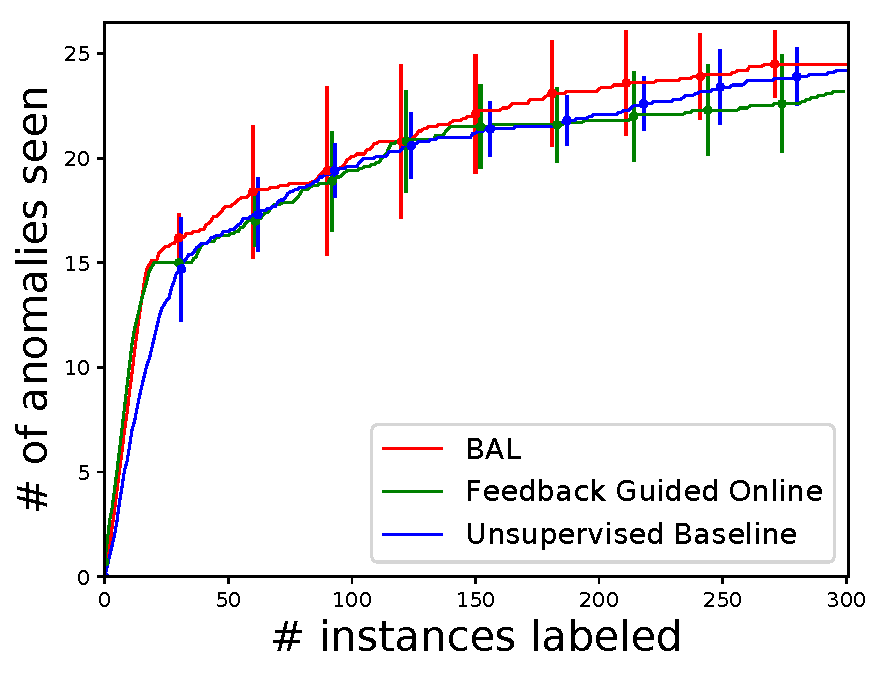
\includegraphics[width=\textwidth]{fbonline/num_seen-abalone.pdf}
		\caption{Abalone}
		\label{fig:angles_abalone}
	\end{subfigure}
	~
	\begin{subfigure}[b]{0.23\textwidth}
		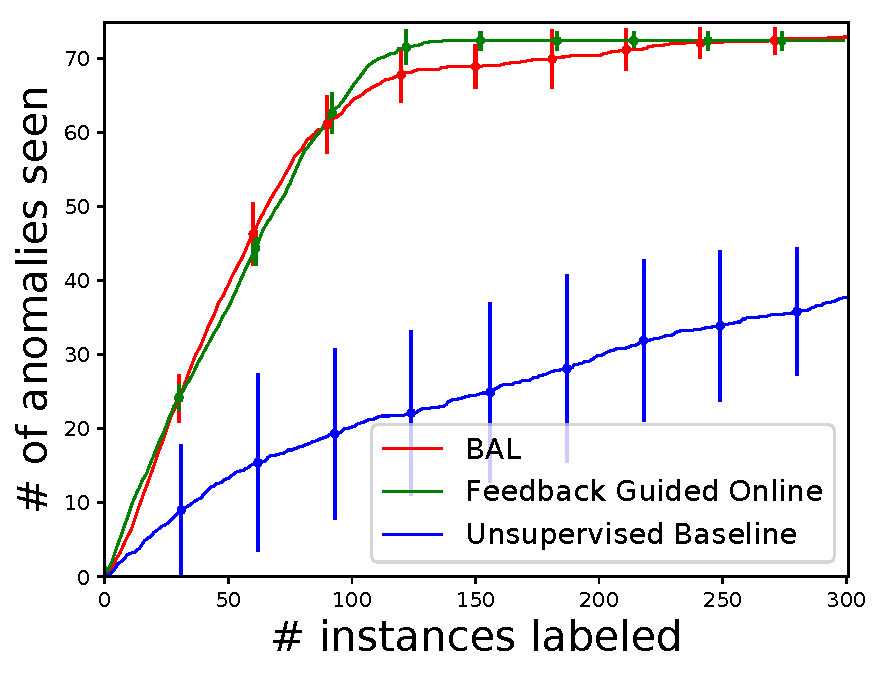
\includegraphics[width=\textwidth]{fbonline/num_seen-ann_thyroid_1v3.pdf}
		\caption{ANN-Thyroid}
		\label{fig:angles_ann_thyroid_1v3}
	\end{subfigure}
	\begin{subfigure}[b]{0.23\textwidth}
		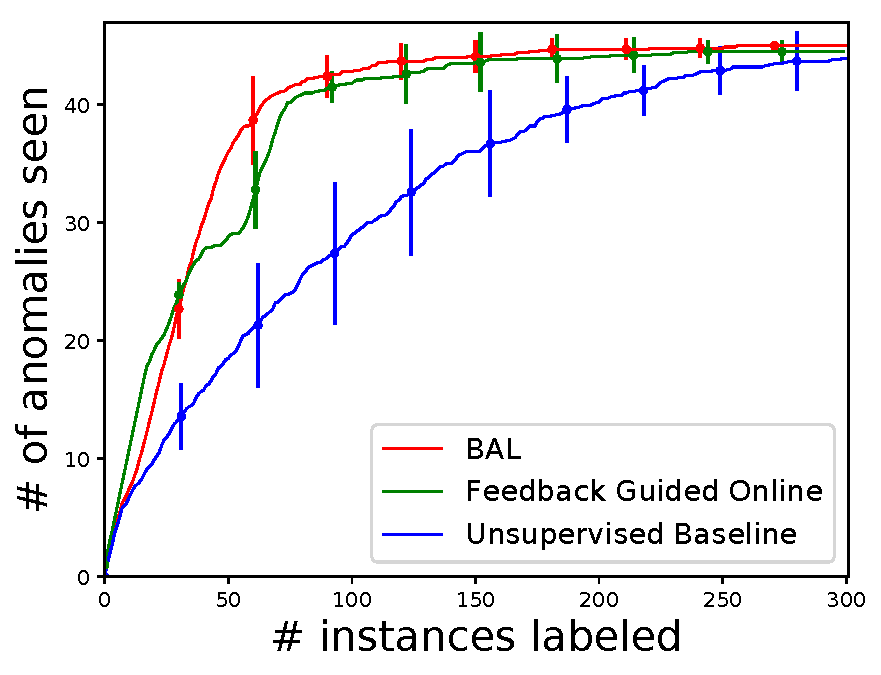
\includegraphics[width=\textwidth]{fbonline/num_seen-cardiotocography_1.pdf}%
		\caption{Cardiotocography}
		\label{fig:angles_cardiotocography}
	\end{subfigure}
	~
	\begin{subfigure}[b]{0.23\textwidth}
		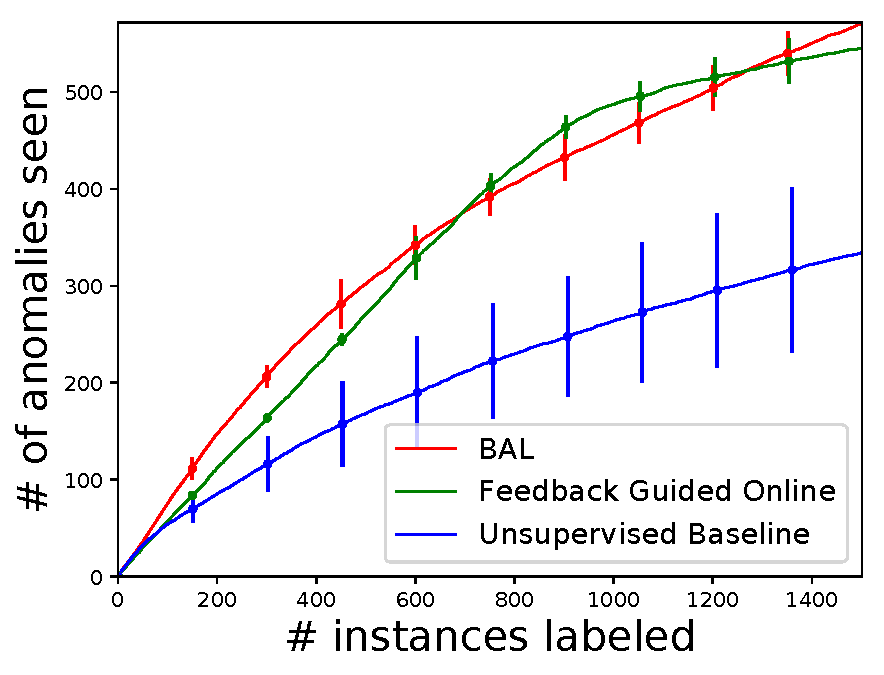
\includegraphics[width=\textwidth]{fbonline/num_seen-electricity.pdf}
		\caption{Electricity}
		\label{fig:angles_electricity}
	\end{subfigure} \\
	\begin{subfigure}[b]{0.23\textwidth}
		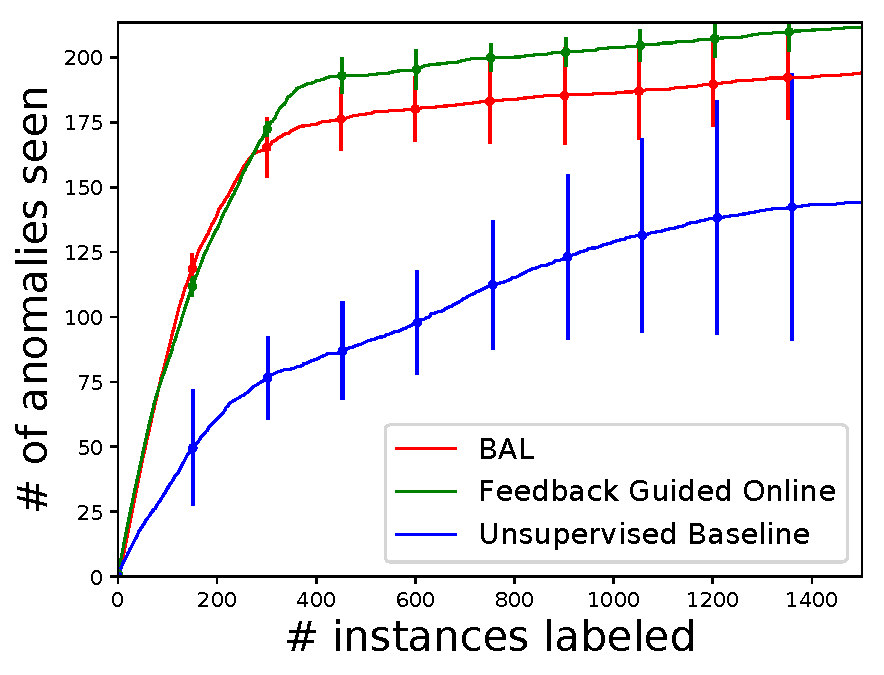
\includegraphics[width=\textwidth]{fbonline/num_seen-mammography.pdf}
		\caption{Mammography}
		\label{fig:angles_mammography}
	\end{subfigure}
	\begin{subfigure}[b]{0.23\textwidth}
		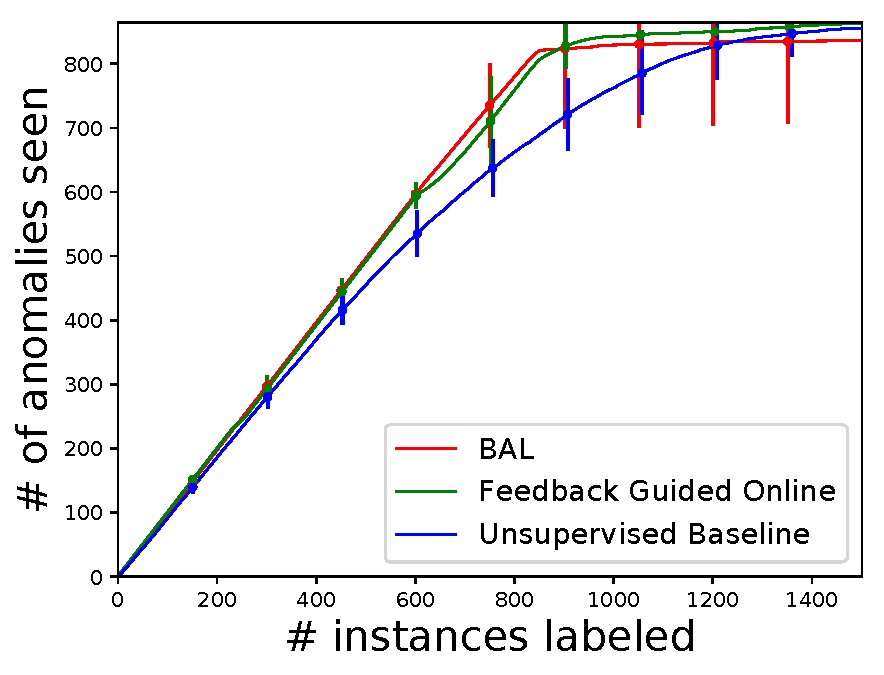
\includegraphics[width=\textwidth]{fbonline/num_seen-shuttle_1v23567.pdf}
		\caption{Shuttle}
		\label{fig:angles_shuttle}
	\end{subfigure}
	\begin{subfigure}[b]{0.23\textwidth}
		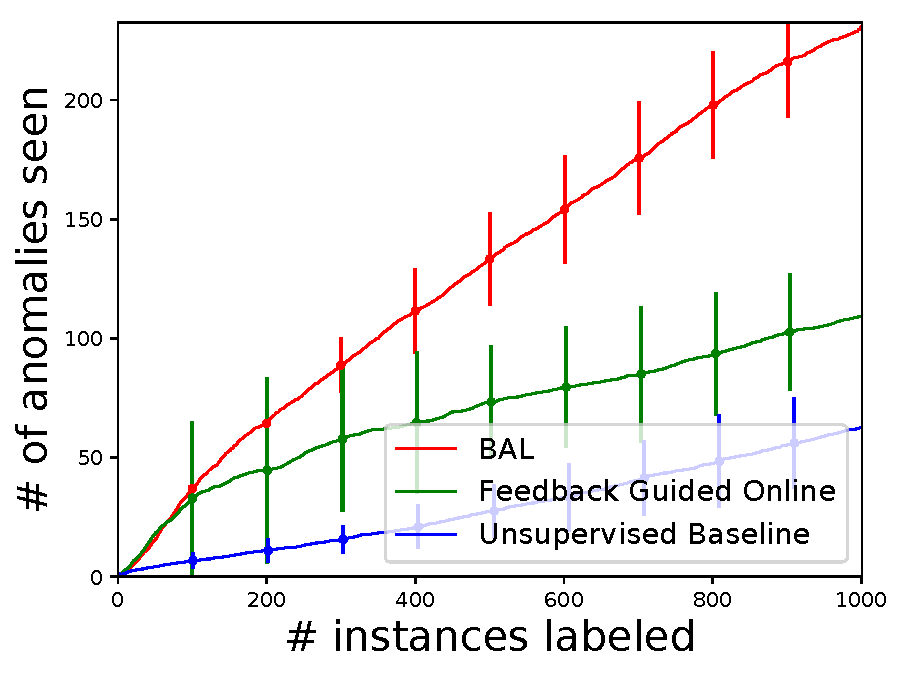
\includegraphics[width=\textwidth]{fbonline/num_seen-weather.pdf}
		\caption{Weather}
		\label{fig:angles_weather}
	\end{subfigure}
	\begin{subfigure}[b]{0.23\textwidth}
		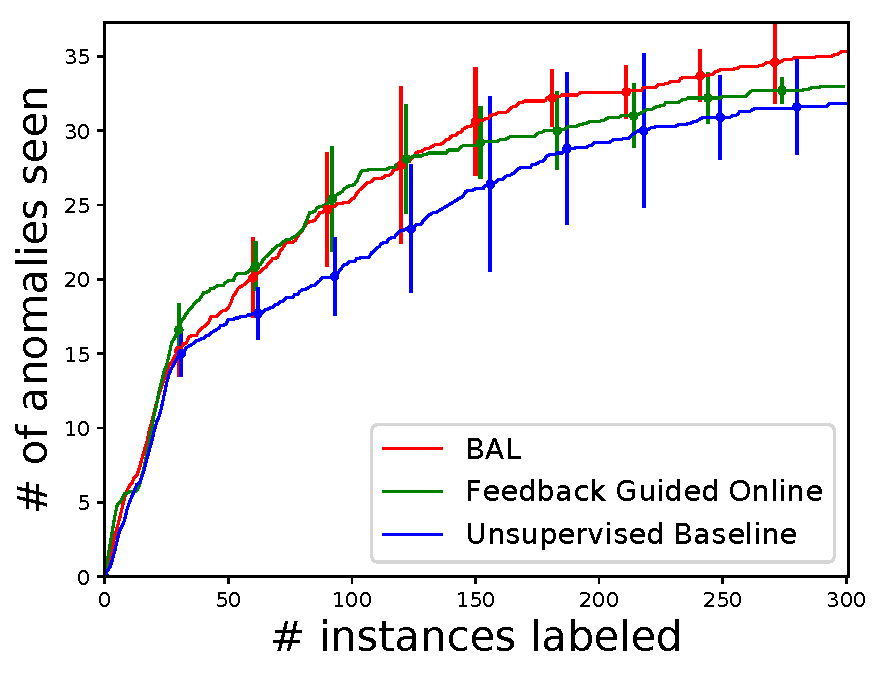
\includegraphics[width=\textwidth]{fbonline/num_seen-yeast.pdf}
		\caption{Yeast}
		\label{fig:angles_yeast}
	\end{subfigure} \\[-1ex]
	\caption{Comparison with Siddiqui et al. 2018. \texttt{BAL} is the tree-based model implemented in this codebase and employs the AAD loss (anomalies score higher than $\tau$-th quantile score and nominals lower). \texttt{Feedback Guided Online} employs the linear loss in Siddiqui et al. 2018. \texttt{Unsupervised Baseline} is the unsupervised Isolation Forest baseline. Both seem to perform similar on most datasets. While \texttt{BAL} has slightly poor accuracy on \textit{Mammography} than \texttt{Feedback Guided Online}, \texttt{BAL} performs much better on \textit{Weather}.}
	\label{fig:fbonline_all}
\end{figure}

\end{document}
